\documentclass[a4paper]{article}
\usepackage[utf8]{vietnam}
\usepackage{graphicx}
\usepackage{amssymb}
\usepackage{amsmath}
\usepackage{scrextend}

\usepackage{times}

\usepackage{listings}
\usepackage{tvietlistings}
\usepackage{xcolor}

%New colors defined below
\definecolor{codegreen}{rgb}{0,0.6,0}
\definecolor{codegray}{rgb}{0.5,0.5,0.5}
\definecolor{codepurple}{rgb}{0.58,0,0.82}
\definecolor{backcolour}{rgb}{0.95,0.95,0.92}

%Code listing style named "mystyle"
\lstdefinestyle{mystyle}{
	backgroundcolor=\color{backcolour},   commentstyle=\color{codegreen},
	keywordstyle=\color{magenta},
	numberstyle=\tiny\color{codegray},
	stringstyle=\color{codepurple},
	basicstyle=\ttfamily\footnotesize,
	breakatwhitespace=false,         
	breaklines=true,                 
	captionpos=b,                    
	keepspaces=true,                 
	numbers=left,                    
	numbersep=5pt,                  
	showspaces=false,                
	showstringspaces=false,
	showtabs=false,                  
	tabsize=2
}

%"mystyle" code listing set
\lstset{style=mystyle}



\title{BIỄU DIỄN TRI THỨC\\ Bài tập 2}
\author{Nhóm 07}
\date{May 29th, 2021}

\begin{document}
	\maketitle
	\begin{center}
		\Large{\textbf{Bài 2 - Bài toán điều chế các chất hóa học}}
	\end{center}
	\section*{Câu a: Tổ chức lưu trữ cho miền tri thức} 
	
	Với phạm vi bài toán, miền tri thức thu thập sẽ nằm trong giới hạn đủ để giải quyết yêu cầu bài toán bao gồm những phương trinh hóa học cần thiết để điều chế \texttt{Na$_2$SO$_4$}, \texttt{H$_2$SO$_4$}, \texttt{HCl} và \texttt{Na} từ \texttt{S}, \texttt{H$_2$O},và \texttt{NaCl} như:\\
	
	
	\texttt{NaCl} = \texttt{Na} = \texttt{Cl$_2$}  
	
	
	\texttt{Na} + \texttt{H$_2$SO$_4$} = \texttt{Na$_2$SO$_4$} + \texttt{SO$_2$} + \texttt{H$_2$O}\\
	
	Sau khi được thu thập, những tri thức này cần được lưu trữ trong tập tin văn bản có cấu trúc \textbf{txt} gồm những quy ước về nguyên tố, hợp chất hóa học, cũng như mối quan hệ giữa chất điều chế và chất được điều chế giúp máy tính hiểu và tính toán được.
		
	\begin{figure}[h]
	\centering
	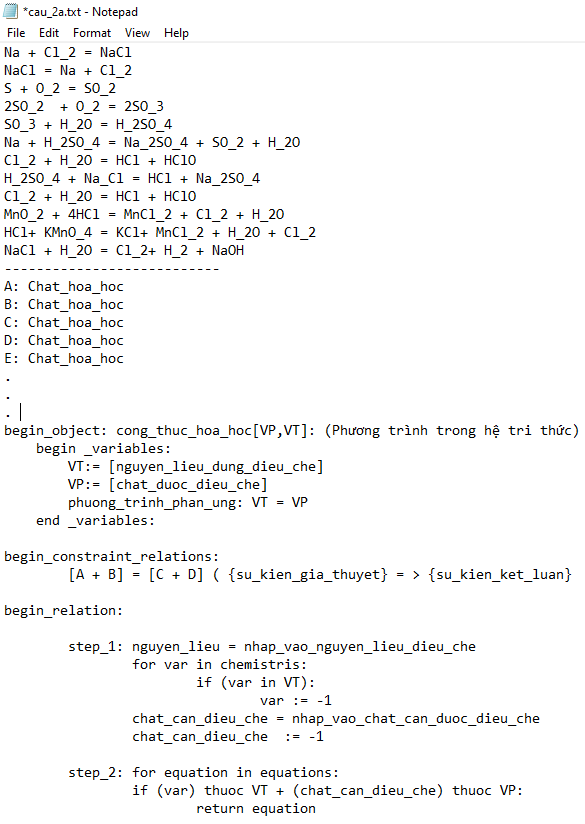
\includegraphics[width=.46\linewidth]{2a_luutru.PNG}  
	\caption{Tổ chức lưu trữ cho miền tri thức điều chế hóa chất}
	\label{}
	\end{figure}


	\section*{Câu b}
	Trình bày thuật giải
	\begin{lstlisting}[language=Python, caption=Thuật giải mạng ngữ nghĩa điều chế]
		def solve(self):
			#Cờ đề truy vết
			flag = True
			while flag:
				flag = False
				print('self.equations', len(self.equations))
				print('self.steps', len(self.steps))
				#Duyệt từng phương trình
					for equation in self.equations:
						#Lấy chất điều chế bên VT phương trình
						known_var = self.get_known_vars(equation)
						#Nếu như 1 node (chất) có thể điều chế được (khác -1)
						if known_var != -1:
							#Kích hoạt node có thể điều chế được
							self.active_var(known_var)
							#Tiến thành lưu lại pt có thể điều chế
							self.add_step(known_var, equation)
							flag = True
							# Kiểm tra xem đã giải bài toán thành công chưa?
							if self.is_success():
								temp = []
								solutions = temp
								# Trả về lời giải đến đích
									for step in self.steps:
										solutions.append(step)
									return [True, solutions]
				# Nếu không giải được trả về yêu cầu thêm thông tin, tri thức
				return [False, "Bài toán không thể giải, hãy bổ sung thêm thông tin hoặc tri thức."]
	\end{lstlisting}
	
	\section*{Câu c}
	Cài đặt chương trình

\end{document}